\documentclass{article}
\usepackage[utf8]{inputenc}
\usepackage{natbib}
\usepackage{amsmath}
\usepackage{geometry}
\geometry{textwidth=7in}
\usepackage{physics}
\usepackage[english]{babel}
\usepackage{enumitem}
\usepackage{graphicx}
\usepackage[colorinlistoftodos]{todonotes}
\usepackage{listings}
\usepackage{color}

\definecolor{dkgreen}{rgb}{0,0.6,0}
\definecolor{gray}{rgb}{0.5,0.5,0.5}
\definecolor{mauve}{rgb}{0.58,0,0.82}

\lstset{frame=tb,
  language=Java,
  aboveskip=3mm,
  belowskip=3mm,
  showstringspaces=false,
  columns=flexible,
  basicstyle={\small\ttfamily},
  numbers=none,
  numberstyle=\tiny\color{gray},
  keywordstyle=\color{blue},
  commentstyle=\color{dkgreen},
  stringstyle=\color{mauve},
  breaklines=true,
  breakatwhitespace=true,
  tabsize=3
}
\begin{document}
\begin{titlepage}
\vspace*{5 cm}

\centering
{\LARGE  University of Oxford\par}
\vspace*{3 cm}

{\Huge \bf Finite Differences}\\[0.2\baselineskip]

\vspace*{2\baselineskip}
\scshape
 MSc in Mathematical Finance\\
\today\par
\vspace*{2\baselineskip}
\vfill
\end{titlepage}

\begin{enumerate}
\item We want to find the explicit Euler central difference scheme for the PDE:
\[\pdv{V}{t} + \frac{1}{2}Y(S^2\pdv[2]{V}{S} + 2\xi\rho{S}\pdv{V}{S}{Y} + \xi^2\pdv[2]{V}{Y}) + rS\pdv{V}{S} + \kappa(\theta -Y)\pdv{V}{Y} - rV = 0\]\
\newline 
Discretising the PDE, we get
\begin{align*}
\frac{V^{m}_{i,j}-V^{m-1}_{i,j}}{\Delta{t}} + Y_ji^2\frac{V^m_{i+1,j}-2V^m_{i,j}+V^m_{i-1,j}}{2} +  ij\xi\rho\frac{V^m_{i+1,j+1}+V^m_{i-1,j-1}-V^m_{i-1,j+1}-V^m_{i+1,j-1}}{4} \\
+ \xi^2j\frac{V^m_{i,j+1}-2V^m_{i,j}+V^m_{i,j-1}}{2\Delta{Y}} + ri\frac{V^m_{i+1,j}-V^m_{i-1,j}}{2} + \kappa(\theta-Y_j)\frac{V^m_{i,j+1}-V^m_{i,j-1}}{2\Delta{Y}} - rV^m_{i,j} = 0
\end{align*}
Setting the subject to $V^{m-1}_{i,j}$, 
\begin{align*}
V^{m-1}_{i,j} = A^m_{i,j}V^m_{i,j} + C^m_{i,j}V^m_{i-1,j} + D^m_{i,j}V^m_{i+1,j} + E^m_{i,j}V^m_{i,j-1} + F^m_{i,j}V^m_{i,j+1} \\
+B^m_{i,j}(V^m_{i+1,j+1}+V^m_{i-1,j-1}-V^m_{i-1,j+1}-V^m_{i+1,j-1})
\end{align*}
where the coefficients are:
\[A^m_{i,j} = 1 - \Delta{t}(r+i^2Y_j+\frac{\xi^2j}{\Delta{Y}})\]
\[B^m_{i,j} = \frac{1}{4} ij\xi\rho\Delta{t}\]
\[C^m_{i,j} = \Delta{t}(\frac{Y_ji^2}{2} - \frac{ir}{2})\]
\[D^m_{i,j} = \Delta{t}(\frac{Y_ji^2}{2} + \frac{ir}{2})\]
\[E^m_{i,j} = \Delta{t}(\frac{\xi^2j}{2\Delta{Y}} - \frac{\kappa(\theta-Y_j)}{2\Delta{Y}})\]
\[F^m_{i,j} = \Delta{t}(\frac{\xi^2j}{2\Delta{Y}} + \frac{\kappa(\theta-Y_j)}{2\Delta{Y}})\] 

The boundary conditions for the scheme cover the maximum and minimum values of S, Y and t. They are:
\begin{flalign}
&\ V(S_i,Y_j,T) = max(K-S_i,0) &&\\
&\ V(0,Y_j,t_m) = Ke^{-rt_m} &&\\
&\ \pdv{V}{t} (S,0,t) + rS\pdv{V}{S} (S,0,t) +  \kappa\theta\pdv{V}{Y} (S,0,t)- rV(S,0,t) = 0 &&\\
&\ \pdv{V(\infty, Y_j, t_m)}{S} = 0 &&\\
&\ \pdv{V(S_i, \infty, t_m)}{Y} = 0 &&\\
\end{flalign}
The first condition is at maturity when the option value equals the payoff. It is used as the final condition in the explicit scheme. The second condition is the boundary when $S=0$ which is when the option price is simply the discounted value of the strike, K, at time t. The third condition is the boundary when $Y=0$ which is obtained by setting Y to 0 in the option pricing PDE. For the boundary $S\rightarrow \infty$, we examine the payoff which is equal to 0 on the interval $S>=K$. Thus it follows that $\pdv{V}{S} = 0$ when $S\rightarrow \infty$. When considering the boundary $Y\rightarrow \infty$, we use the Neumann  condition stated in (5). \\
\\
We can rewrite the above in the form:
\begin{align*}
V^{m-1}_{i,j} = V^m_{i,j} - \Delta{t}(a^m_{i,j}V^m_{i,j} - c^m_{i,j}V^m_{i-1,j} - d^m_{i,j}V^m_{i+1,j} - e^m_{i,j}V^m_{i,j-1} - f^m_{i,j}V^m_{i,j+1} \\
-b^m_{i,j}(V^m_{i+1,j+1}+V^m_{i-1,j-1}-V^m_{i-1,j+1}-V^m_{i+1,j-1}))
\end{align*}
where we redefine the coefficients as :
\[a^m_{i,j} = r+i^2Y_j+\frac{\xi^2j}{\Delta{Y}}\]
\[b^m_{i,j} = \frac{1}{4} ij\xi\rho\]
\[c^m_{i,j} = (\frac{Y_ji^2}{2} - \frac{ir}{2})\]
\[d^m_{i,j} = (\frac{Y_ji^2}{2} + \frac{ir}{2})\]
\[e^m_{i,j} = (\frac{\xi^2j}{2\Delta{Y}} - \frac{\kappa(\theta-Y_j)}{2\Delta{Y}})\]
\[f^m_{i,j} = (\frac{\xi^2j}{2\Delta{Y}} + \frac{\kappa(\theta-Y_j)}{2\Delta{Y}})\]

If we consider a stencil of points to calculate $V^{m-1}_{i,j}$, using the discretised equation and the above coefficients, we get:
\[
\begin{bmatrix}
b_{i,j} & -f_{i,j} & -b_{i,j}\\
-c_{i,j}&a_{i,j}&-d_{i,j}\\
-b_{i,j}&-e_{i,j}&b_{i,j}
\end{bmatrix}
\star
\begin{bmatrix}
V^m_{i-1,j+1} &V^m_{i,j+1} & V^m_{i+1,j+1}\\
V^m_{i-1,j}&V^m_{i,j}&V^m_{i+1,j}\\
V^m_{i-1,j-1}&V^m_{i,j-1}&V^m_{i+1,j-1}
\end{bmatrix}
\] 
To write this in matrix form, we first write $V^m$ as a vector:
\[V^m=[V^m_{11},V^m_{21},V^m_{31},...,V^m_{I1},V^m_{21},V^m_{22},...,V^m_{I2},...,V^m_{IJ}]^T\]\
We construct A as an $IJ \times IJ$ sparse diagonal matrix of the form,
\[\begin{bmatrix}
C_1 & N_1 & 0 & 0 &0&\cdots&0 \\
S_2 & C_2 & N_2 & 0 &0&\cdots&0 \\
0 & S_3 & C_3 & N_3 &0&\cdots&0 \\
\vdots & \ddots & \ddots & \ddots & \ddots&\ddots&\vdots \\
0&\cdots&0&S_{J-2}&C_{J-2}&N_{J-2}&0 \\
0&\cdots&\cdots&\cdots&S_{J-1}&C_{J-1}&N_{J-1}\\
0&\cdots&\cdots&\cdots&\cdots&S_{J}&C_{J}\\
\end{bmatrix}\] 
where each of C, N and S are tridiagonal $I \times I$ matrices. \\

We define C, N and S as sparse tridiagonal matrices each covering part of the stencil. \\
C covers the east, west and central coefficients:
\[
C_j = 
\begin{bmatrix}
    a_{1,j} & -d_{1,j} &0&\cdots&0 \\
    -c_{2,j} & a_{2,j} & -d_{1,j} &\cdots&0 \\
    \vdots & \ddots & \ddots & \ddots &\vdots \\
    0&\cdots&-c_{i-1,j} & a_{i-1,j} & -d_{i-1,j}\\
    0&\cdots&\cdots&-c_{i,j} & a_{i,j}\\
\end{bmatrix}\] 
S covers the southwest, south and southeast coefficients:
\[
S_j = 
\begin{bmatrix}
    -e_{1,j} & b_{1,j} & 0&\cdots&0 \\
    -b_{2,j} & -e_{2,j} & b_{2,j} &\cdots&0 \\
    \vdots & \ddots & \ddots & \ddots & \vdots \\
    0&\cdots&-b_{i-1,j} & -e_{i-1,j} & b_{i-1,j}\\
    0&\cdots&\cdots&-b_{i,j} & -e_{i,j}\\
\end{bmatrix}\] 
N covers the northwest, north and northeast coefficients:
\[
N_j = 
\begin{bmatrix}
    -f_{1,j} & -b_{1,j} & 0 &\cdots&0 \\
    b_{2,j} & -f_{2,j} & -b_{2,j} &\cdots&0 \\
    \vdots & \ddots & \ddots&\ddots&\vdots \\
    0&\cdots&b_{i-1,j} & -f_{i-1,j} & -b_{i-1,j}\\
    0&\cdots&\cdots&b_{i,j} & -f_{i,j}\\
\end{bmatrix}\] 

Thus we can now express the scheme in the form $V^{m-1} = (I-\Delta{t}A)V^m$.

Thus we get,
\[
\begin{bmatrix}
V^{m-1}_{11}\\
V^{m-1}_{21}\\
\vdots\\
V^{m-1}_{I,1}\\
V^{m-1}_{12}\\
\vdots \\
V^{m-1}_{I2}\\
\vdots\\
V^{m-1}_{IJ}
\end{bmatrix}
=
\begin{bmatrix}
V^{m}_{11}\\
V^{m}_{21}\\
\vdots\\
V^{m}_{I,1}\\
V^{m}_{12}\\
\vdots \\
V^{m-1}_{I2}\\
\vdots\\
V^{m}_{IJ}
\end{bmatrix}
-
\Delta{t}\begin{bmatrix}
a^{m}_{1,1} & -d^{m}_{1,1} & 0 & \cdots &-f^{m}_{1,1}&-b^{m}_{1,1}&0&0&\cdots&0 \\
-c^m_{2,1} & a^m_{2,1} & -d^m_{2,1} & \cdots &b^m_{2,1}&-f^m_{2,1}&-b^{m}_{2,1}&0&\cdots&0 \\
\vdots & \ddots & \ddots & \ddots & \ddots&\ddots&\ddots&\ddots&\ddots&\vdots \\
0&\cdots & -c^m_{I,1} & a^m_{I,1} & 0&\cdots&b^m_{I,1}&-f^{m}_{I,1}&0&\cdots \\
-e^{m}_{1,2} & b^{m}_{1,2} & 0 & \cdots &a^{m}_{1,2}&-d^{m}_{1,2}&0&\cdots&-f^m_{1,2}&\cdots \\
\vdots & \ddots & \ddots & \ddots & \ddots&\ddots&\ddots&\ddots&\ddots&\vdots \\
0&\cdots & -b^m_{I,2} & -e^m_{I,2} & 0&\cdots&a^m_{I,2}&-d^{m}_{I,2}&0&\cdots \\
\vdots & \ddots & \ddots & \ddots & \ddots&\ddots&\ddots&\ddots&\ddots&\vdots \\
0&\cdots&0&\cdots & -b^m_{I,J} & -e^m_{I,J} & 0&\cdots&-c^m_{I,J}&a^{m}_{I,J}\\
\end{bmatrix}\
\begin{bmatrix}
V^{m}_{11}\\
V^{m}_{21}\\
\vdots\\
V^{m}_{I,1}\\
V^{m}_{12}\\
\vdots \\
V^{m-1}_{I2}\\
\vdots\\
V^{m}_{IJ}
\end{bmatrix}
\] 

\item 
To find the price of the option, we need to discretise the boundary conditions detailed above. The discrete boundaries are at $i=0, j=0, i=I+1, j=J+1$ as A is an $IJ \times IJ$ matrix and covers the rest of the internal points. These are the discretised conditions:
\begin{flalign*}
&\ V^M_{i,j} = max(K-i\Delta{S},0) &&\\
&\ V^m_{0,j} = Ke^{-rm\Delta{t}} &&\\
&\ \frac{V^m_{i,0}-V^{m-1}_{i,0}}{\Delta{t}} + ri \frac{V^m_{i+1,0} - V^m_{i-1,0}}{2} + \kappa\theta\frac{V^m_{i,1} - V^m_{i,0}}{\Delta{Y}} -rV^m_{i,0}=0&&\\
&\ \frac{V^m_{I+1,j} - V^m_{I,j}}{\Delta{S}} = 0 &&\\
&\ \frac{V^m_{i,J+1} - V^m_{i,J}}{\Delta{Y}} = 0 &&\\
\end{flalign*}
\textbf{Final Condition}\\
The first condition is used as the final condition in the scheme and we work backwards from it to calculate the option price at previous timesteps.\\

\textbf{Dirichlet boundary at $S=0$}\\
The second condition where $S=0/i=0$ is a Dirichlet boundary condition. To handle this, the following missing terms need to be added to the solution where $i=1$:
\[c^m_{1,j}V^m_{0,j} + b^m_{1,j}(V^m_{0,j-1} - V^m_{0,j+1})\]
Since $V^m_{0,j}$ is constant as it is the discounted time-value of K, the term to be added reduces to $c^m_{1,j}V^m_{0,j}$. \\

\textbf{Boundary at $Y=0$}\\
The third condition where $Y=0/j=0$ is a discretised PDE and we need an explicit scheme to handle it. We get:
\[V^{m-1}_{i,0} = V^m_{i,0}(1-\frac{\kappa\theta\Delta{t}}{\Delta{Y}}-r\Delta{t}) + V^m_{i+1,0}\frac{ri\Delta{t}}{2} + V^m_{i+1,0}\frac{-ri\Delta{t}}{2} + \frac{\kappa\theta\Delta{t}}{\Delta{Y}}V^m_{i,0}\]\
We have $V^m_{i,1}$ from the internal grid values and can calculate $V^m_{i,0}$ using an explicit scheme. This then turns into a dirichlet boundary where we add the following terms to the solution where $j=1$:
\[e^m_{i,1}V^m_{i,0} + b^m_{i,1}(V^m_{i-1,0} - V^m_{i+1,0})\]

\textbf{Neumann boundary at $S=\infty/i=I+1$}\\
From the boundary condition, we have $V^m_{I+1,j} = V^m_{I,j}$. 
\[d^m_{I,j}V^m_{I+1,j}  + b^m_{I,j}(V^m_{I+1,j+1} - V^m_{I+1,j-1}) = d^m_{I,j}V^m_{I,j}  + b^m_{I,j}(V^m_{I,j+1} - V^m_{I,j-1})\]\
We need to modify the matrix accordingly with the above terms. The dirichlet boundary covers the term for $V^m_{0,I+1}$ and combining the two derivative boundary conditions we have $V_{I+1,J+1}=V_{I,J}$. \\

\textbf{Neumann boundary at $Y=\infty/j=J+1$}\\
From the boundary condition, we have $V^m_{i,J+1} = V^m_{i,J}$. 
\[f^m_{i,J}V^m_{i,J+1}  + b^m_{i,J}(V^m_{i+1,J+1} - V^m_{i-1,J+1}) = f^m_{i,J}V^m_{i,J}  + b^m_{i,J}(V^m_{i+1,J} - V^m_{i-1,J}) \]\
We need to modify the matrix accordingly with the above terms. The term for $V_{I+1,J+1}=V_{I,J}$ is already taken care of above. 

On implementing the explicit scheme using the calculated matrix and the boundary conditions, I get the answer 0.0665 for the price of the option at $t=0$, $S_0=1.3$ and $Y_0=0.01$ with I, J and M set to 4. On experimenting with the values of I, J and M, I could see that the scheme became unstable for very large grids over smaller timesteps. It did not blow up in cases where the number of timesteps, M, was increasing with I and J.  This is in accordance with the conditional stability of the explicit scheme which gives a reasonable solution provided the number of timesteps is sufficiently large, given an increasing number of grid points. 

Code used to generate this is in Appendix 1. 

\item We need to show that the scheme $P^{m+1} = (I-\Delta{t}A^T)P^m$ is a consistent approximation for the forward Kolmogorov PDE associated with the Heston model. \\

If we take the transpose of A, we get:
\[
\begin{bmatrix}
a^{m}_{1,1} & -c^{m}_{2,1} & 0 & \cdots &-e^{m}_{1,2}&-b^{m}_{2,2}&0&0&\cdots&0 \\
-d^m_{1,1} & a^m_{2,1} & -c^m_{3,1} & \cdots &b^m_{1,2}&-e^m_{2,2}&-b^{m}_{3,2}&0&\cdots&0 \\
\vdots & \ddots & \ddots & \ddots & \ddots&\ddots&\ddots&\ddots&\ddots&\vdots \\
0&\cdots & -d^m_{I-1,1} & a^m_{I,1} & 0&\cdots&b^m_{I-1,2}&-f^{m}_{I,2}&0&\cdots \\

-f^{m}_{1,1} & b^{m}_{2,1} & 0 & \cdots &a^{m}_{1,2}&-c^{m}_{2,2}&0&\cdots&-f^m_{1,3}&\cdots \\
\vdots & \ddots & \ddots & \ddots & \ddots&\ddots&\ddots&\ddots&\ddots&\vdots \\
0&\cdots & -b^m_{I-1,1} & -f^m_{I,1} & 0&\cdots&a^m_{I-1,2}&-c^{m}_{I,2}&0&\cdots \\
\vdots & \ddots & \ddots & \ddots & \ddots&\ddots&\ddots&\ddots&\ddots&\vdots \\
0&\cdots&0&\cdots & -b^m_{I-1,J-1} & -f^m_{I,J-1} & 0&\cdots&-d^m_{I-1,J}&a^{m}_{I,J}\\
\end{bmatrix}\
\] 
where the coefficients a,b,c,d,e,f are defined on page 2. \\

Expressing this as a triadiagonal matrix,

\[\begin{bmatrix}
C_1^T & S_2^T & 0 & 0 &0&\cdots&0 \\
N_1^T & C_2^T & S_3^T & 0 &0&\cdots&0 \\
0 & N_2^T & C_3^T & S_4^T &0&\cdots&0 \\
\vdots & \ddots & \ddots & \ddots & \ddots&\ddots&\vdots \\
0&\cdots&\cdots&\cdots&N^T_{J-2}&C^T_{J-1}&S^T_{J}\\
0&\cdots&\cdots&\cdots&\cdots&N^T_{J-1}&C^T_{J}\\
\end{bmatrix}\] 

Converting this to an equation,
\begin{align*}
P^{m+1}_{i,j} = P^m_{i,j} - \Delta{t}(a^m_{i,j}P^m_{i,j} - c^m_{i+1,j}P^m_{i+1,j} - d^m_{i-1,j}P^m_{i-1,j} - e^m_{i,j+1}P^m_{i,j+1} - f^m_{i,j-1}P^m_{i,j-1} \\
-b^m_{i+1,j+1}P^m_{i+1,j+1}-b^m_{i-1,j-1}P^m_{i-1,j-1}+b^m_{i-1,j+1}P^m_{i-1,j+1}+b^m_{i+1,j-1}P^m_{i+1,j-1})
\end{align*}
Substituting the coefficients we calculated earlier, 
\begin{align*}
P^{m+1}_{i,j} = P^{m}_{i,j}(1 - r\Delta{t} - i^2Y_j\Delta{t} - \frac{\xi^2\Delta{t}}{\Delta{Y}} ) + P^{m}_{i-1,j}\Delta{t}(\frac{r(i-1)}{2} +\frac{Y_j(i-1)^2}{2}) + P^{m}_{i+1,j}\Delta{t}(-\frac{r(i+1)}{2} +\frac{Y_j(i+1)^2}{2})\\
P^m_{i,j-1}\Delta{t}(\frac{\kappa\theta}{2\Delta{Y}} + \frac{\xi^2}{2\Delta{Y}} - \frac{\kappa}{2}(j-1)) + P^m_{i,j+1}\Delta{t}(-\frac{\kappa\theta}{2\Delta{Y}} + \frac{\xi^2}{2\Delta{Y}} + \frac{\kappa}{2}(j+1)) +\frac{\xi\rho\Delta{t}}{4}(i+1)(j+1)P^m_{i+1,j+1} \\
+\frac{\xi\rho\Delta{t}}{4}(i-1)(j-1)P^m_{i-1,j-1} -\frac{\xi\rho\Delta{t}}{4}(i+1)(j-1)P^m_{i+1,j-1} -\frac{\xi\rho\Delta{t}}{4}(i-1)(j+1)P^m_{i-1,j+1}
\end{align*}

Converting this to a discretised PDE,
\begin{align*}
\frac{P^{m+1}_{i,j}-P^{m}_{i,j}}{\Delta{t}} + \frac{r}{2}((i+1)P^m_{i+1,j}-(i-1)P^m_{i-1,j}) + \frac{\kappa\theta}{2\Delta{Y}}(P^m_{i,j+1}-P^m_{i,j-1}) - \frac{\kappa}{2}((j+1)P^m_{i,j+1}-(j-1)P^m_{i,j-1}) \\
- \frac{1}{2}Y_j((i+1)^2P^m_{i+1,j}-2i^2P^m_{i,j}+(i-1)^2P^m_{i-1,j})  - \frac{\xi^2}{2\Delta{Y}}((j+1)P^m_{i,j+1}-2jP^m_{i,j}+(j-1)P^m_{i,j-1})\\
- \frac{\xi\rho}{4}((i+1)(j+1)P^m_{i+1,j+1}+(i-1)(j-1)P^m_{i-1,j-1}-(i-1)(j+1)P^m_{i-1,j+1}-(i+1)(j-1)P^m_{i+1,j-1}) - rP^m_{i,j} = 0
\end{align*}
From this, we recover the equation:
\[\pdv{P}{t} + r\pdv{(SP)}{S} + \kappa\pdv{((\theta - Y)P)}{Y} -\frac{1}{2}\pdv[2]{(YS^2P)}{S} -\frac{\xi^2}{2}\pdv[2]{(YP)}{Y} - \rho\xi\pdv{(SYP)}{S}{Y} -rP= 0\]\
with initial condition $P(S,V,0) = \delta(S-S_0)\delta(V-V_0)$. \\
This is the forward Kolmogorov equation associated with the Heston model. Thus we have shown that the scheme $P^{m+1} = (I-\Delta{t}A^T)P^m$ is an approximation for it.\\
\\
The truncation error for this scheme is defined as:
\begin{align*}
\tau^m_{i,j} = P^{m+1}_{i,j} - P^m_{i,j} + \Delta{t}(a^m_{i,j}P^m_{i,j} - c^m_{i+1,j}P^m_{i+1,j} - d^m_{i-1,j}P^m_{i-1,j} - e^m_{i,j+1}P^m_{i,j+1} - f^m_{i,j-1}P^m_{i,j-1} \\
-b^m_{i+1,j+1}P^m_{i+1,j+1}-b^m_{i-1,j-1}P^m_{i-1,j-1}+b^m_{i-1,j+1}P^m_{i-1,j+1}+b^m_{i+1,j-1}P^m_{i+1,j-1})
\end{align*}
The scheme is consistent of order $(p,q,r)$ if, for sufficiently smooth solutions P, $\tau^m_{i,j} = O(\Delta{Y}^p, \Delta{S}^q, \Delta{t}^r)$. \\
On calculating the Taylor expansions:
\[P_{i+1,j} = P_{i,j} + \Delta{S}\pdv{P_{i,j}}{S}+ \frac{1}{2}(\Delta{S})^2\pdv[2]{P_{i,j}}{S}+ \frac{1}{6}(\Delta{S})^3\pdv[3]{P_{i,j}}{S} + \frac{1}{24}(\Delta{S})^4\pdv[2]{P_{i,j}}{S}\]\
\[P_{i-1,j} = P_{i,j} - \Delta{S}\pdv{P_{i,j}}{S} + \frac{1}{2}(\Delta{S})^2\pdv[2]{P_{i,j}}{S}- \frac{1}{6}(\Delta{S})^3\pdv[3]{P_{i,j}}{S} + \frac{1}{24}(\Delta{S})^4\pdv[2]{P_{i,j}}{S}\]\
We get similar expressions for $P_{i,j+1}$ and $P_{i,j-1}$ substituting the S for Y. \\
For the mixed derivatives we get:
\begin{align*}
P_{i+1,j+1} = P_{i,j} + \Delta{S}\pdv{P_{i,j}}{S}+ \Delta{Y}\pdv{P_{i,j}}{Y} + 
\frac{1}{2}[(\Delta{S})^2\pdv[2]{P_{i,j}}{S} + (\Delta{Y})^2\pdv[2]{P_{i,j}}{Y} + 2\Delta{S}\Delta{Y}\pdv{P_{i,j}}{S}{Y} +  \\ 
(\Delta{S})^2\pdv[2]{P_{i,j}}{S} ]
+ \frac{1}{6} [(\Delta{S})^3\pdv[3]{P_{i,j}}{S} +( \Delta{Y})^3\pdv[3]{P_{i,j}}{Y} + 3\Delta{S}(\Delta{Y})^2\pdv{P_{i,j}}{S}{Y^2}+ 
3\Delta{Y}(\Delta{S})^2\pdv[3]{P_{i,j}}{S^2}{Y} ] + ..
\end{align*}
Similar expressions for the other mixed derivatives. \\
The approximation to the time derivative is also needed:
\begin{align*}
\frac{P^{m+1}_{i,j}-P^{m}_{i,j}}{\Delta{t}}  = \pdv{P^m_{i,j}}{t} + \frac{\Delta{t}}{2}\pdv[2]{P^m_{i,j}}{t} 
\end{align*}
On substituting these terms into the discretised PDE above, we derive the consistency order to be $O( \Delta{S}^2, \Delta{Y}^2, \Delta{t},)$.

\item In the modifications, we have to consider:
\begin{enumerate}
\item The matrix A has to be transposed.
\item Since this is a forward equation, we can no longer use the final condition as the payoff. We have the initial condition $P(S,V,0) = \delta(S-S_0)\delta(V-V_0)$ where $S_0=1.3, Y_0=0.01$. However, the Dirac mass is not well-behaved and needs to be approximated to avoid numerical issues arising from lack of smoothness. \\
A Dirac delta distribution is the limit of a normal distribution as the variance tends to 0. Thus the initial condition can be approximated using a bivariate normal distribution:
\[P^0_{i,j} = \frac{1}{2\pi\sigma_s\sigma_y}\exp{-\frac{1}{2\sigma^2_s}(S-S_0)^2 - \frac{1}{2\sigma^2_y}(Y-Y_0)^2}\]\
 where $\sigma^2_s$ and $\sigma^2_s$ are set to 0.001.
\item Boundary conditions 
\begin{itemize}
\item Boundary at $j=0/Y=0$\\
The variance process $Y_t$ is strictly positive if the market parameters follow Feller's condition:
\[2\kappa\theta - \xi^2 >0\]
Plugging in $\kappa = 2, \theta=0.015, \xi=0.2$:
\[2*2*0.015 - 0.2^2 = 0.02 > 0\]
Thus there is 0 probability of $Y_t$ reaching 0 and we can set the boundary, $P^m_{i,0}$, to 0.\\
\item Boundary at $j=J+1, i=I+1$\\
We use the Neumann boundary conditions we defined for the explicit scheme earlier. 
\end{itemize}
\end{enumerate}
I experimented for some values of I, J and M to calculate the transition probabilities and have plotted results for some combinations below.
\begin{figure}[!htbp]
    \centering
    \hspace*{-2cm}
    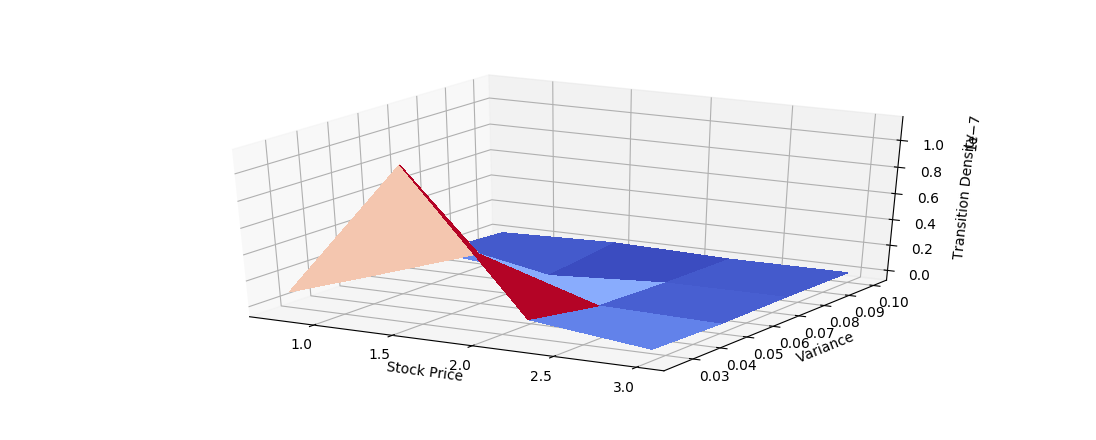
\includegraphics[width=1.1\columnwidth]{/Users/tanvipotdar/Projects/Advanced-Numerical-Methods/fd/td_4}
    \caption{Transition probability density for (S,Y) for I, J and M set to 4}
 \end{figure}

\begin{figure}[!htbp]
    \centering
    \hspace*{-2cm}
    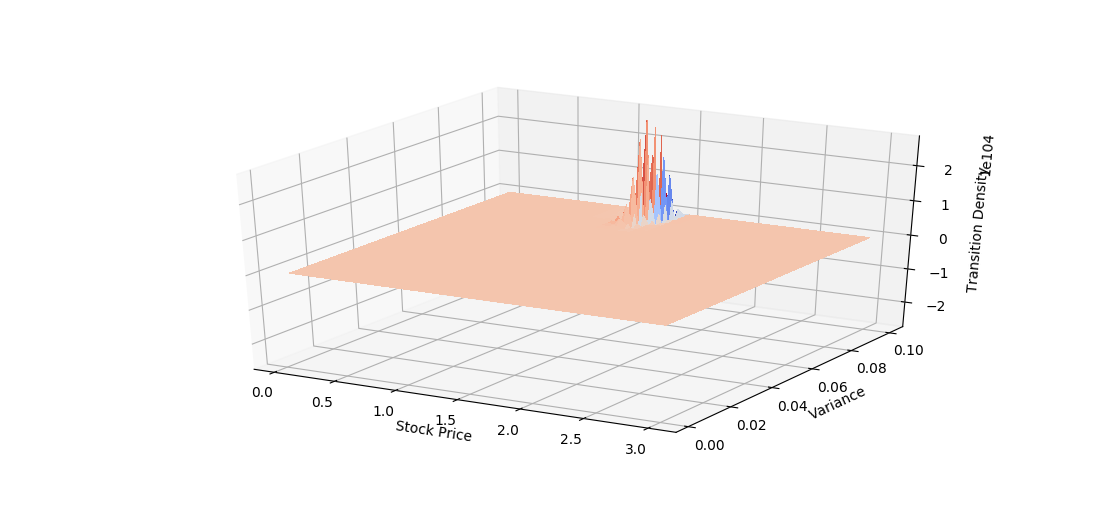
\includegraphics[width=1.1\columnwidth]{/Users/tanvipotdar/Projects/Advanced-Numerical-Methods/fd/td_64}
    \caption{Transition probability density for (S,Y) for I, J and M set to 64}
\end{figure}

\item We can write,
\[\sigma^2(s,t) = \mathbf{E}[Y_t|S_t=s] = \frac{\int^{\infty}_{0}YP(S,Y,t)dY}{\int^{\infty}_{0}P(S,Y,t)dY}\]\
where P(S,Y,t) is the transition probability density function. To calculate $\sigma^2(s,t)$, we need to approximate the integrals above. 
\[\sigma^2(S_i,t_m) =\frac{\sum_{j=1}^{J}Y_jP(S_i,Y_j,t_m)dY}{\sum_{j=1}^{J}P(S_i,Y_j,t_m)dY}\]\
I used Simpson's quadrature rule for numerical integration and calculated a matrix of $\sigma^2(s,t)$ of length $M \times I$ with $\sigma^2_{m,i}$ corresponding to the variance at $S_i, t_m$. I have plotted the results for the variance for a few different combinations of I, J and M. The code for this is in Appendix 2. 
\begin{figure}[!htbp]
    \centering
    \hspace*{-2cm}
    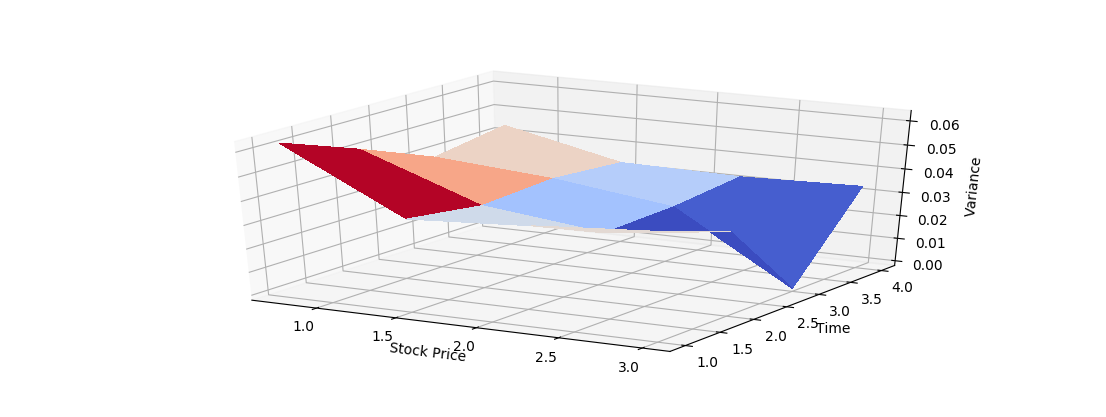
\includegraphics[width=1.1\textwidth]{/Users/tanvipotdar/Projects/Advanced-Numerical-Methods/fd/var_4}
    \caption{Heston local variance over stock price and time with I, J and M set to 4}
\end{figure}

\begin{figure}[!htbp]
    \centering
    \vspace*{-0.2cm}
    \hspace*{-2cm}
    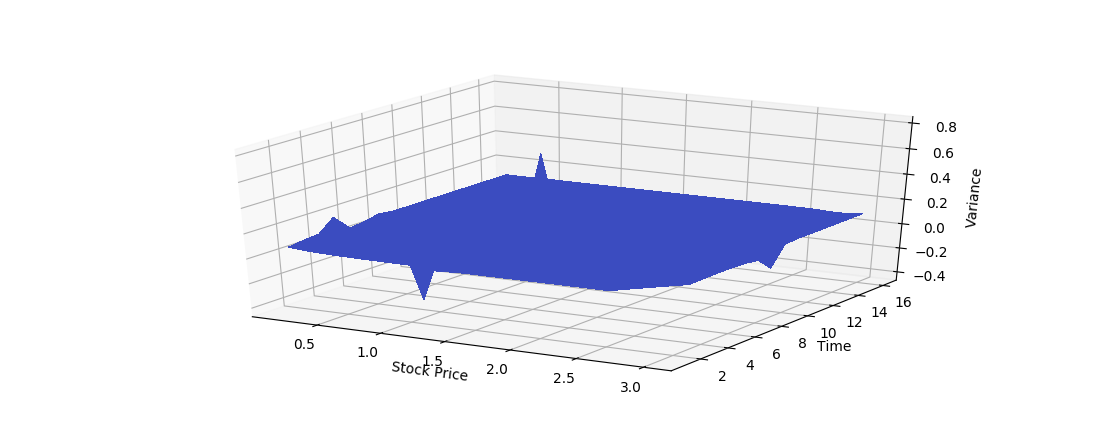
\includegraphics[width=1.1\textwidth]{/Users/tanvipotdar/Projects/Advanced-Numerical-Methods/fd/var_16}
    \caption{Heston local variance over stock price and time with I, J and M set to 16}
\end{figure}

\begin{figure}[!htbp]
    \centering
    \vspace*{-0.7cm}
    \hspace*{-2cm}
    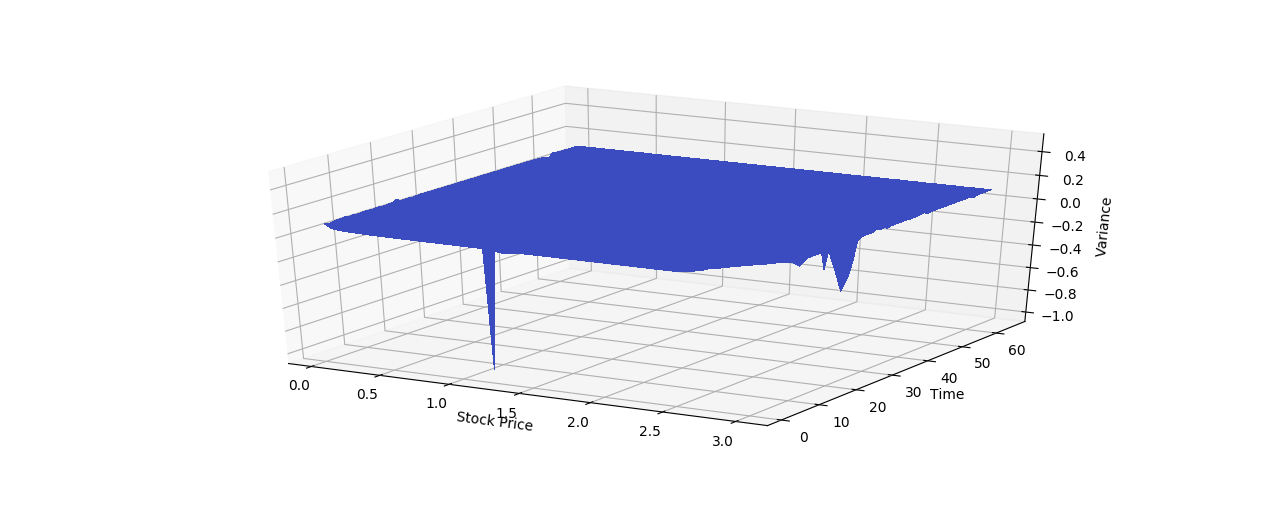
\includegraphics[width=1.1\textwidth]{/Users/tanvipotdar/Projects/Advanced-Numerical-Methods/fd/var_64}
    \caption{Heston local variance over stock price and time with I, J and M set to 64}
\end{figure}

\item To verify the finite difference solution, we first need to discretise the one-dimensional PDE:
\[\frac{V^{m}_{i,j}-V^{m-1}_{i,j}}{\Delta{t}} + \frac{1}{2}\sigma^2(S_i,t_m)i^2(V^m_{i+1,j} -2V^m_{i,j}+V^m_{i-1,j}) + \frac{ir}{2} (V^m_{i+1,j} - V^m_{i-1,j}) -rV^m_{i,j}=0\]\
In order to use an explicit finite difference scheme, we need to calculate $V^{m-1}$ using $V^m$:
\[V^{m-1}_{i,j} = V^{m}_{i,j}(1-r\Delta{t}-\sigma^2(S_i,t_m)\Delta{t}) + V^m_{i+1,j}(\frac{1}{2}\sigma^2(S_i,t_m)i^2 + \frac{ir\Delta{t}}{2}) + V^m_{i-1,j}(\frac{1}{2}\sigma^2(S_i,t_m)i^2 - \frac{ir\Delta{t}}{2})\]\
\[V^{m-1}_{i,j} = A^m_{i,j}V^{m}_{i,j} + B^m_{i,j}V^m_{i+1,j}+ C^m_{i,j}V^m_{i-1,j}\]\
On implementing this using an explicit finite difference scheme, I get 0.072 as the option price given an initial stock price $S_0$ of 1.3. This is implemented in the file transition\textunderscore{density}.py. The solution I got in part 2 was 0.067. Thus, we can verify that both solutions round up to 0.07.
\end{enumerate}
\newpage
\section{Appendix}
\subsection{Code for question 2 of the assignment to compute the price of the put option}
\begin{lstlisting}
import numpy as np
from scipy.sparse import spdiags
from scipy.interpolate import interp2d


def create_stock_price_grid(Smin, Smax, I):
    S = np.linspace(Smin, Smax, I + 1)[1:]
    return S

def create_vol_grid(Ymin, Ymax, J):
    Y = np.linspace(Ymin, Ymax, J + 1)[1:]
    Y.shape = (J, 1)
    return Y

def get_payoff_values_at_maturity(K, S, J):
    V = map(lambda x: max(K - x, 0), S)
    V = np.concatenate([V] * J, axis=0)
    return V

def calculate_stencil_coefficients(i, j, Y, J, dY, dt, r=0.03, kappa=2, xi=0.2, rho=-0.2, theta=0.015):
    term1 = np.matmul(j, i * i)
    term2 = np.matmul(j, i)

    j = np.array(map(lambda x: [x[0]] * J, j))
    Y = np.array(map(lambda x: [x[0]] * J, Y))

    j = np.array(map(lambda x: [x[0]] * J, j))
    Y = np.array(map(lambda x: [x[0]] * J, Y))

    term_c = 1 - dt * (term1 * dY + j * xi ** 2 / dY + r)
    term_e = 0.5 * dt * (term1 * dY + i * r)
    term_w = 0.5 * term1 * dY * dt - 0.5 * dt * i * r

    term_n = 0.5 * dt * (xi ** 2 * j / dY + (kappa / dY) * (theta - Y))
    term_s = 0.5 * dt * (xi ** 2 * j / dY - (kappa / dY) * (theta - Y))
    term_b = 0.25 * xi * rho * term2 * dt

    return term_c, term_e, term_w, term_n, term_s, term_b

def get_matrix(term_c, term_e, term_w, term_n, term_s, term_b, I, J):
    matrix = np.zeros((J, I, J, I))
    for i in range(I):
        data = np.array([term_w[i], term_c[i], term_e[i]])
        mat = spdiags(data, [1, 0, -1], J, I).toarray().transpose()
        mat[I-1][I-1]+=term_e[i][-1]
        matrix[i][i] = mat

    for i in range(I - 1):
        data = np.array([-term_b[i], term_n[i], term_b[i]])
        mat = spdiags(data, [1, 0, -1], J, I).toarray().transpose()
        mat[I-1][I-1]+=term_b[i][-1]
        matrix[i][i + 1] = mat

    for i in range(1, I):
        data = np.array([term_b[i], term_s[i], -term_b[i]])
        mat = spdiags(data, [1, 0, -1], J, I).toarray().transpose()
        mat[I-1][I-1]+=-term_b[i][-1]
        matrix[i][i - 1] = mat

    jmax_data = np.array([-term_b[I-1], term_n[I-1], term_b[I-1]])
    jmax_mat = spdiags(jmax_data, [1, 0, -1], J, I).toarray().transpose()
    matrix[J-1][I-1]+=jmax_mat


    A = matrix.swapaxes(1, 2).reshape((I ** 2, J ** 2))
    return A

def get_smin_boundary_values(V, term_w, initial_val, I):
    w_terms = term_w.copy()
    for i in range(I):
        w_terms[i][1:].fill(0)
    w_terms = w_terms.reshape((V.shape))
    smin_boundary = w_terms * initial_val
    return smin_boundary


def get_jmin_boundary_values(V, I, J, i, r, kappa, theta, dt, dY, jmins, initial_val, term_s, term_b):
    payoff_values_for_j_equals_one = V[:J]
    const = (kappa * theta * dt)/dY
    V_i_1 = const * payoff_values_for_j_equals_one 

    a = np.array([1- r*dt - const]*I)   
    b = (r*i*dt)/2
    b = b[0]

    data = np.array([-b, a, b])
    mat = spdiags(data, [1, 0, -1], I, I).toarray().transpose()

    jmin_vals = jmins[:J]
    jmin_vals = np.matmul(mat, jmin_vals) + V_i_1
    jmin_vals[0]+=-b[0]*initial_val
    jmin_vals[-1]+=b[0]*jmin_vals[-1]

    jmin_boundaries = np.append(initial_val, np.append(jmin_vals, jmin_vals[-1]))
    jmin_diff = jmin_boundaries[:-2] - jmin_boundaries[2:]

    jmins[:J] = term_s[0]*jmin_vals + term_b[0]*jmin_diff
    return jmins


def compute_price(I=4, J=4, M=4):
    r = 0.03
    rho = -0.2
    xi = 0.2
    kappa = 2
    theta = 0.015
    K = 1.2
    T = 3

    Smin = 0
    Ymin = 0
    Smax = 3
    Ymax = 0.1

    S0 = 1.3
    Y0 = 0.01

    S = create_stock_price_grid(Smin, Smax, I)
    Y = create_vol_grid(Ymin, Ymax, J)
    V = get_payoff_values_at_maturity(K, S, J)

    dS = (Smax - Smin) / float(I)
    dY = (Ymax - Ymin) / float(J)
    i = S / dS
    i.shape = (1,I)
    j = Y / dY
    dt = T/float(M)

    term_c, term_e, term_w, term_n, term_s, term_b = calculate_stencil_coefficients(i, j, Y, J, dY, dt)
    A = get_matrix(term_c, term_e, term_w, term_n, term_s, term_b, I, J)

    jmin_boundary_values = np.zeros(V.shape)
    jmin_boundary_values[:J] = V[:J]
    for m in range(M, 0, -1):
        initial_val = K * np.exp(-r * (T - m * dt))
        smin_boundary_values = get_smin_boundary_values(V, term_w, initial_val, I)

        V_prev = V.copy()

        V = np.matmul(A,V) + smin_boundary_values + jmin_boundary_values
        jmin_boundary_values = get_jmin_boundary_values(V_prev, I, J, i, r, kappa, theta, dt, dY, jmin_boundary_values, initial_val, term_s, term_b)

    f = interp2d(S, Y, V.reshape(I, J))
    return f(S0, Y0)
\end{lstlisting}
\newpage
\subsection{Code for question 4,5 and 6 of the assignment to calculate and plot transition density and local variance }
\begin{lstlisting}
from heston import create_stock_price_grid, create_vol_grid, calculate_stencil_coefficients, get_matrix
from mpl_toolkits.mplot3d import Axes3D
import matplotlib.pyplot as plt
from matplotlib import cm
from matplotlib.ticker import LinearLocator, FormatStrFormatter
import numpy as np
from scipy.stats import norm, gamma
from scipy.interpolate import interp1d
from scipy.integrate import simps, cumtrapz
from scipy.sparse import spdiags

r = 0.03
rho = -0.2
xi = 0.2
kappa = 2
theta = 0.015
K = 1.2
T = 1
Smax = 3
Ymax = 0.1
S0 = 1.3
Y0 = 0.01


def get_initial_values(S0, Y0, S, Y, dt, I, J):
    stock_var = 0.001
    vol_var = 0.001
    term1 = 1 / (2 * 3.14 * np.sqrt(stock_var) * np.sqrt(vol_var))
    s_terms = map(lambda x: -(1 / (2 * stock_var)) * (x - S0) ** 2, S)
    y_terms = map(lambda x: -(1 / (2 * vol_var)) * (x - Y0) ** 2, Y)
    y_terms = np.concatenate(y_terms, axis=0)
    return term1 * np.array(map(np.exp, [y + s for y in y_terms for s in s_terms]))


def get_min_vol_boundary_values(P, I, dY, dt):
    """
    Need to fulfil the zero flux condition when Y=0/j=0.
    Generate vector of P(i,0) values and then multiples by relevant coefficients as shown below
    To be added to j=1/P(i,1) terms for P(i, j-1) values: term_n(i,0)P(i,0) + term_b(i-1,0)P(i-1,0) + term_b(i+1,0)P(i+1,0)
    term_b = 0 when j = 0 thus return [term_n(1,0)P(1,0), term_n(2,0)P(2,0), ...] of len I*J
    """
    const = xi ** 2 / (2 * dY * kappa * theta)
    term_n_for_min_j = (dt * kappa * theta) / (2 * dY)
    min_vol_values = np.zeros(P.shape)
    min_vol_values[:I] = term_n_for_min_j * const * P[:I]
    return min_vol_values


def calculate_transition_density_and_var(P, S, Y, I, J, M):
    dt = T / float(M)
    dS = Smax / float(I)
    dY = Ymax / float(J)
    i = S / dS
    i.shape = (1, I)
    j = Y / dY

    term_c, term_e, term_w, term_n, term_s, term_b = calculate_stencil_coefficients(i, j, Y, J, dY, dt)
    A = get_matrix(term_c, term_e, term_w, term_n, term_s, term_b, I, J)
    A = A.transpose()

    var = np.zeros((M,I))

    for m in range(M):
        P = np.matmul(A, P)
        var[m] = compute_var_for_timestep(P,Y,I,J,dY)

    return P, var


def compute_var_for_timestep(P, Y, I, J, dY):
    P = P.reshape(I,J)
    Y.shape = (1,J)
    y = Y[0]
    var = simps(P.transpose()*y,y,axis=1)/simps(P,y, axis=0)
    return var


def plot_variance(S, I, M, var):
    s_grid = np.meshgrid(S, S)[0]
    t_grid = np.array([[x]*I for x in range(1,M+1)])
    fig = plt.figure(figsize=(10,7))
    ax = fig.gca(projection='3d')
    ax.set_xlabel('Stock Price')
    ax.set_ylabel('Time')
    ax.set_zlabel('Variance')
    ax.plot_surface(s_grid, t_grid, var, cmap=cm.coolwarm, linewidth=0, antialiased=False)
    plt.show()


def plot_transition_density(S, Y, I, J, P):
    s_grid = np.meshgrid(S, S)[0]
    y_grid = np.meshgrid(Y, Y)[0].transpose()
    p_grid = P.reshape(I, J)
    fig = plt.figure(figsize=(10,7))
    ax = fig.gca(projection='3d')
    ax.set_xlabel('Stock Price')
    ax.set_ylabel('Variance')
    ax.set_zlabel('Transition Density')
    ax.plot_surface(s_grid, y_grid, p_grid, cmap=cm.coolwarm, linewidth=0, antialiased=False)
    plt.show()


def create_plots(I=4, J=4, M=4):
    dt = T / float(M)
    S = create_stock_price_grid(0, Smax, I)
    Y = create_vol_grid(0, Ymax, J)
    initial_p = get_initial_values(S0, Y0, S, Y, dt, I, J)
    P, var = calculate_transition_density_and_var(initial_p, S, Y, I, J, M)
    plot_transition_density(S, Y, I, J, P)
    plot_variance(S, I, M, var)


def compute_price(I=4, J=4, M=4):
    T=3;
    r=0.03;
    S = create_stock_price_grid(0, Smax, I)
    Y = create_vol_grid(0, Ymax, J)
    dt = T / float(M)
    dS = Smax / float(I)
    i = S / dS

    V = map(lambda x: max(K - x, 0), S)

    initial_p = get_initial_values(S0, Y0, S, Y, dt, I, J)
    _, vol = calculate_transition_density_and_var(initial_p, S, Y, I, J, M)

    for m in range(M, 0, -1):
        initial_val = K * np.exp(-r * (T - m * dt))
        sigma = vol[m-1]
        term1=sigma*i
        term1=term1*term1
        term2=r*i

        A=0.5*dt*(term1-term2)
        B=1-dt*(term1+r)
        C=0.5*dt*(term1+term2)

        data = np.array([C, B, A])
        mat = spdiags(data, [-1, 0, 1], J, I).toarray().transpose()
        V=np.matmul(mat,V)
        V[0] += initial_val * A[0]

    f = interp1d(S, V)
    return f(S0)
\end{lstlisting}
\end{document}